\documentclass[12pt,aspectratio=169,svgnames]{beamer}

\usepackage{modules/cgs}

\begin{document} \maketitle

\begin{frame}{Содержание}
	\tableofcontents
\end{frame}

\section{O-нотация}

\subsection{Определение}

\begin{frame}{Идея \(O\)}
	Пусть некоторая программа принимает на вход данные. \\
	Она, скорее всего, работает тем дольше, чем больше \\
	данных поступило на вход. Мы хотим оценить время работы \\
	программы, сравнивая его с известными функциями \(\bn \to \bn\).
\end{frame}


\begin{frame}{Определение из анализа}
\begin{defn}
	Функции \(f,\ g\,\colon\ \br \to \br\). Говорят, что
		\[f(x) = O(g(x)),\ \ \text{если}\ \ \exists\,C\ \forall\,x\ 
			|f(x)| \le C \cdot |g(x)|. \]
\end{defn}
\end{frame}


\begin{frame}{Определение для нас} \ \\
\begin{defn}
	Время работы программы составляет \(O(f(n))\), если \\
	существует \(C\): для входа {\it размера \(n\)} количество операций \\
	составит не более \(f(n) \cdot C\).
\end{defn}

\begin{itemize}
	\item Какие операции считаются в данном определении, \\
	      обычно известно из контекста.
	\item Если вход состоит из {\it одного числа,} размер \\
	      входа равен 1, вне зависимости от величины числа.
\end{itemize}
\end{frame}

\subsection{Максимум в массиве}

\begin{frame}{Поиск наибольшего элемента в массиве} \ \\
\begin{task}
	Дан массив из \(n\) чисел, найти в нём наибольший элемент.
\end{task}

Отсмотрим все элементы по порядку, храня наибольший \\
отсмотренный элемент. Мы обращаемся к каждому элементу \\
по разу, поэтому \(O(n)\). Быстрее, очевидно, нельзя.
	\begin{center} \tikz{
	\foreach \x / \t in {
	   -4.5 / {[},  -4 / 1,  -3 / 4,  -2 / 4,  -1 / 2,  0 / 8,
	    4.5 / {]},   1 / 1,   2 / 6,   3 / 9,   4 / 8
	} {\draw (0.9*\x,0) node{\t};}

	\draw[HotPink] (0.9,-1.1) node{8}
		(0.7,-1.1) node[left]{{\tiny max to date:}};
	\draw[->,HotPink] (0.9,-0.7)--(0.9,-0.35);
	\draw[HotPink] (1.1,-0.85) rectangle ++(-1.8,-0.5);
} \end{center}

\end{frame}

\subsection{Элемент в отсортированном массиве}

\begin{frame}{Наличие элемента в отсортированном массиве} \ \\
\begin{task}
	Дан массив \(M\) из \(n\) чисел, они упорядочены по возрастанию. \\
	Дано число \(k\)~— проверить, есть ли оно в \(M\).
\end{task}

Сравним \(k\) и элемент в середине \(M\)~— назовём его \(m\). \\
Если \(m>k\), ищем в первой половине массива. Иначе во второй.
	\begin{center} \tikz{
	\foreach \x / \t in {
	   -4.5 / {[},  -4 / 1,  -3 / 2,  -2 / 3,  -1 / 5,  0 / 8,
	    4.5 / {]},   1 / 13,   2 / 21,   3 / 34,   4 / 55
	} {\draw (0.9*\x,0) node{\t};}

	\draw[HotPink] (0,-0.9)--(0,-0.5)
		(-0.65,-0.7) node[left]{{\scriptsize �����?}}
		(0.65,-0.7) node[right]{{\scriptsize ��� �����?}};
	\draw[HotPink,->] (-0.2,-0.7) -- ++(-0.35,0);
	\draw[HotPink,->] (0.2,-0.7) -- ++(0.35,0);
} \end{center}

\end{frame}

\begin{frame}{Как оценить время работы}
	Пусть \(T(n)\)~— время работы на массиве из \(n\) элементов. Тогда
	\[ T(n) = 1 + T\lr*{\frac{n}{2}}.\]

	Отсюда \[ T(n) = O\lr*{\log_2 \lr*{n}}.\]
\end{frame}

\subsection{Количество комнат на корабле}

\begin{frame}{Количество комнат на космическом корабле} \ \\
\begin{task}
	Космический корабль в форме кольца разделён на \(n\) \\
	одинаковых комнат, в которых горит или не горит свет. \\
	Можно переходить между соседними комнатами, \\
	включать или выключать свет. Найти \(n\).
\end{task} \medskip

\begin{center} \tikz{
	\torship001100101 \me5
} \end{center}
\end{frame}


\begin{frame}{Простое решение}
	Процедура \(\text{проход}\lr*{k}\)~— пройти на \(k\) комнат вперёд, включая \\
	в каждой комнате свет (может быть что угодно).

	Потом пройти на \(k\) комнат назад, выключая в каждой \\
	комнате свет (должен быть включен).

\begin{center} \tikz{
	\torship011110101 \me2
	\draw[thick,Violet,->] (-95:1.6) arc (-95:-205:1.6);
} \hspace{2cm} \tikz{
	\torship000000101 \me5
	\draw[thick,Violet,<-] (-95:1.6) arc (-95:-205:1.6);
} \end{center}
\end{frame}


\begin{frame}{Оценка времени}
	Выполним \(\text{проход}\lr*{1}, \text{проход}\lr*{2}, \text{проход}\lr*{3}, \ldots\)

	В какой-то момент мы вернёмся, чтобы выключить свет \\
	в первой комнате, а он уже будет там выключен. \\
	Значит, мы прошли полный круг.
	\[2 \cdot (1+2+\ldots+n) = O\lr*{n^2}\text{\ \ переходов.}\]
\end{frame}


\begin{frame}{Решение за линейное время {\it (Doubling search)}}
	Пусть \(2^{k-1} \le n < 2^k\).

	Выполним \(\text{проход}\lr*{1}, \text{проход}\lr*{2},\ldots,
	\text{проход}\lr*{2^i},\ldots\)

	Каждый раз длина прохода увеличивается в два раза. \\
	В какой-то момент на обратном пути мы придём \\
	в комнату, свет в которой уже выключен.
	\[2 \cdot \lr*{1+2+4+\ldots+2^k}\ =\ 2 \cdot \lr*{2^{k+1}-1}\ 
		\le\ 8 \cdot n\ =\ O(n).\]
\end{frame}

\subsection{Алгоритм Беллмана — Форда}

\begin{frame}{Алгоритм Беллмана — Форда}
\begin{task}
	Дан граф \(G = \lr*{V,E}\), на рёбрах расставлены неотрицательные \\
	веса. Выбрана \(v \in V\), найти наименьшие веса путей от \(v\) \\
	до каждой из остальных вершин.
\end{task}

Изначально \(d(v_i) = +\infty\) для всех \(v_i\).
\end{frame}


\begin{frame}{Идея}
\begin{center}
{\footnotesize \textcolor{white!46!dgray}{Считаем, что все \(d(v_i)\)
	обновляются одновременно.
	В реальности дело чуть лучше.}}
                 \tikz[xscale=0.34,yscale=0.48]{
	\coordsequence
	\cbfnode{1}{0}{0}; \cbfnode{2}{100}{2};
	\cbfnode{3}{100}{4}; \cbfnode{4}{0}{\q};
	\cbfnode{5}{0}{\q}; \cbfnode{6}{0}{\q};
	\edgesequence
} \hspace{1.1cm} \tikz[xscale=0.34,yscale=0.48]{
	\coordsequence
	\cbfnode{1}{0}{0}; \cbfnode{2}{0}{2};
	\cbfnode{3}{100}{3}; \cbfnode{4}{100}{6};
	\cbfnode{5}{100}{10}; \cbfnode{6}{100}{11};
	\edgesequence
} \hspace{1.1cm} \tikz[xscale=0.34,yscale=0.48]{
	\coordsequence
	\cbfnode{1}{0}{0}; \cbfnode{2}{0}{2};
	\cbfnode{3}{0}{3}; \cbfnode{4}{0}{6};
	\cbfnode{5}{100}{8}; \cbfnode{6}{100}{10};
	\edgesequence
} \\ [0.35 cm]
\end{center}
\end{frame}


\begin{frame}{Улучшение \(d(v_i)\)}
\begin{center} \begin{algorithmic}
   \For{\(i=1\) to \(|V| - 1\)}
      \ForAll{\(e = (u_1,u_2) \in E\)}
         \If{\(d(u_1) + \text{weight}(e) < d(u_2)\)} \\
            \qquad\qquad \(d(u_2) \leftarrow d(u_1) +  \text{weight}(e)\)
            \Comment{Пытаемся с помощью ребра \(e\)\\ \hfill улучшить путь в \(v_2\)}
         \EndIf
      \EndFor \Comment{Нашли оптимальные пути длины \(\le i\)}
   \EndFor
\end{algorithmic} \end{center}
\end{frame}


\begin{frame}{Асимптотика с несколькими параметрами}
	Время работы оценивается как \(O\lr*{ |V| \cdot |E| }\). \bigskip

	Мы, конечно, знаем, что \(|V| \le |E|+1\) и \(|E| \le |V|^2\), \\
	но зачастую нам нужна точная оценка \\
	относительно обоих параметров входа.
\end{frame}

\subsection{Замечания}

\begin{frame}{Замечания}
\begin{itemize}
	\item \( \log_a n\ \ll\ n^k\ \ll\ a^n \) \bigskip
	\item \( \log_a n\ \sim\ \log_b n \) \bigskip
	\item \( \log_a \lr*{x^k}\ \sim\ \log_a x \)
\end{itemize}
\end{frame}


\section{Задачи, выполнимые за $O(1)$}
\begin{frame}{Некоторые договоренности}

	Для удобства мы будем считать, что точки \alert{в общем положении}

	\begin{itemize}
		\item Никакие 3 из них не лежат на одной прямой.

		\item Никакие 4 из них не лежат на одной окружности.

		\item У них нет общих $x$ и $y$ координат.
	\end{itemize}

	В совокупности это верно почти всегда.\\

\end{frame}

\subsection{Применения аналитической геометрии}

\begin{frame}{Задание фигур уравнениями}

	При работе с геом. объектами удобно задавать их уравнениями

		\begin{itemize}
			\item Прямая:\\

			$\ell\colon ax + by + c = 0$ или $\ell\colon y = kx + b$.\\
			Прямая через точки $A(x_1, y_1), B(x_2, y_2)$:
			\[ \ell\colon \begin{cases} ax_1 + by_1 + c = 0 \\ ax_2 + by_2 + c = 0 \end{cases}\]
			\[ a = y_2 - y_1, \ b = x_1 - x_2, \ c = -(ax_1 + by_1)\]

			\item Окружность:
			\[ (x - x_0)^2 + (y - y_0)^2 = R^2, \text{ где } (x_0, y_0) \text{ — центр, а } R \text{ — радиус} \]
		\end{itemize}

\end{frame}

\begin{frame}{Расстояние от точки до прямой}

	Если прямая задана как  $\ell\colon ax + by + c = 0$, то расстояние от точки $M(x_0, y_0)$ до неё можно рассчитать как
	\[ d(M, \ell) = \frac{\left| ax_0 + by_0 + c \right|}{\sqrt{a^2 + b^2}} \]

	\begin{center}
	\begin{tikzpicture}[scale = 0.64]
	\coordinate[label=left:$M$] (M) at (3,5);
	\draw[fill4, fill = fill4] (3,5) circle (0.07);
	\draw[fill4, fill = fill4] (4,1) circle (0.07);
	\draw[fill4, thick] (0, 0)--(8, 2) node[left, right = 0.05]{$\ell$};
	\draw[fill4, thick] (3, 5)--(4, 1);
	\end{tikzpicture}
	\end{center}

\end{frame}

\subsection{Центр описанной окружности}

\begin{frame}{Центр описанной окружности}

	\vspace{2.5mm}
	\begin{task}

		Дана тройка точек $a, b, c$. Требуется найти центр описанной окружности $\triangle abc$.

	\end{task}

	\begin{center}
		\begin{tikzpicture}[sty/.style={fill = fill4, circle, inner sep=2pt}]
		\coordinate[sty, label=left:$a$] (A) at (0,0); \coordinate[sty,label=right:$b$](B) at (3,1); \coordinate[sty,label=above:$c$](C) at (1,3);
		\draw[thick, fill4] (A)--(B)--(C)--(A);
		\coordinate (T) at ($(A)!1!60:(B)$); \draw [name path=h1, dashed]
		(T)--($(A)!(T)!(B)$); \coordinate (T) at ($(B)!1!60:(C)$);
		\draw [name path=h2, dashed] (T)--($(B)!(T)!(C)$); \draw [name intersections=
		{of=h1 and h2, by=O}]; \node[sty, label=right:$O$] at (O) {};
		\draw[thick, fill5] (O) let \p1=($(O)-(A)$)
		in circle ({veclen(\x1,\y1)});
	   \end{tikzpicture}
	\end{center}

\end{frame}

\begin{frame}{Центр описанной окружности}

	\begin{enumerate}

	    \item Ищем серединные перепендикуляры к $[ac]$ и $[bc]$,\\ как прямые $p_1$ и $p_2$.\\

			  Если $\ell_1\colon y = a_1x + b_1$, а $\ell_2\colon y = a_2 x + b_2$, то $\ell_1 \perp \ell_2 \Leftrightarrow a_1 \cdot a_2 = -1$.\\
			  Находим серединный перпендикуляр к стороне как прямую, проходящую через середину стороны и перпендикулярную ей.

		\item Ищем их пересечение, как решение линейной системы: \\
			$p_1\colon y = \alpha_1 x + \beta, \ p_2\colon y = \alpha_2 x + \beta_2$.\\
		 	\vspace{1mm}
			$\begin{cases} y = \alpha_1 x + \beta_1 \\ y = \alpha_2 x + \beta_2 \end{cases}$

	\end{enumerate}

\end{frame}

\begin{frame}{Смежные задачи}

	Ясно, что очень большое количество задач можно решить совершенно аналогичным образом, например, задачи
	нахождения

	\begin{itemize}

		\item инцентра.

		\item ортоцентра.

		\item  барицентра.
	\end{itemize}
\end{frame}

\subsection{Ориентация и косое произведение}

\begin{frame}{Угол между векторами}

	Рассмотрим вектора $\vec{a} = (x_1, y_1)$ и $\vec{b} = (x_2, y_2)$.
	\[ \langle \vec{a}, \vec{b} \rangle = x_1 x_2 + y_1 y_2 = |\vec{a}||\vec{b}| \cos{\angle{(\vec{a}, \vec{b})}} = \sqrt{x_1^2 + y_1^2}\sqrt{x_2^2 + y_2^2} \cos{\angle(\vec{a}, \vec{b})}\]
	Значит, мы знаем, как найти угол между векторами $\vec{a}$ и $\vec{b}$:
	\[ \angle(\vec{a}, \vec{b}) = \arccos\lr*{\frac{x_1 y_1 + x_2 y_2}{\sqrt{x_1^2 + y_1^2} \sqrt{x_2^2 + y_2^2}}} \]

\end{frame}

\begin{frame}{Косое произведение}

	\begin{defn}

		\alert{Косым произведением} векторов $\vec{a} = (x_1, y_1)$ и $\vec{b} = (x_2, y_2)$ на плоскости будем называть
		\[ \vec{a} \wedge \vec{b} =  \begin{vmatrix} x_1 & y_1 \\ x_2 & y_2  \end{vmatrix} = x_1 y_2 - x_2 y_1\]

	\end{defn}

	Покажем, что $\vec{a} \wedge \vec{b} = |\vec{a}| |\vec{b}| \sin \lr*{\angle \lr*{\vec{a},\vec{b}}}$, где $\angle\lr*{\vec{a}, \vec{b}}$~--- угол
	вращения против часовой стрелки от $\vec{a}$ к $\vec{b}$.

\end{frame}

\begin{frame}{Эквивалентность определений}

	В самом деле, $ \cos \lr*{\angle \lr*{a,b}} = x_1 x_2 + y_1 y_2 / (\sqrt{x_1^2 + y_1^2}\sqrt{x_2^2 + y_2^2})$.
	\begin{multline*} \sin \lr*{\angle \lr*{\vec{a},\vec{b}}} = \sqrt{1 - \cos^2 \lr*{\angle \lr*{\vec{a},\vec{b}}}}) = \sqrt{1 - \frac{(x_1 x_2 + y_1 y_2)^2}{(x_1^2 + y_1^2)(x_2^2 + y_2^2)}} =\\= \sqrt{\frac{x_1^2 x_2^2 + x_1^2 y_2^2 + y_1^2 x_2^2 + y_1^2 y_2^2 - x_1^2 x_2^2 - y_1^2 y_2^2 - 2 x_1 x_2 y_1 y_2 }{(x_1^2 + y_1^2)(x_2^2 + y_2^2)}} \\= \frac{x_1 y_2 - y_1 x_2}{\sqrt{(x_1^2 + y_1^2)}\sqrt{(x_2^2 + y_2^2)}} = \frac{\vec{a} \wedge \vec{b}}{|\vec{a}||\vec{b}|} \end{multline*}

\end{frame}

\begin{frame}{Площадь треугольника}

	Теперь ясно, что $\vec{a} \wedge \vec{b} = 2 S_{\triangle{ABD}}$, где площадь \alert{ориентированная.}

	\begin{center}
	\begin{tikzpicture}
	\coordinate[label=left:$A$] (A) at (0,0); \coordinate[label=left:$B$] (B) at (1,3); \coordinate[label=right:$C$] (C) at (4,3); \coordinate[label=right:$D$] (D) at (3,0);
	\draw[->, fill4, thick] (0,0)--(1,3) node[midway, left = 0.1]{$\vec{a}$};
	\draw[->, fill4, thick] (0,0)--(3,0) node[midway, below = 0.1]{$\vec{b}$};
	\draw[fill4, thick] (1,3)--(3,0);
	\draw[fill4, fill=fill4, fill opacity=0.5, draw opacity = 0] plot coordinates{(0,0) (1,3) (3, 0)}--cycle;
	\draw (A)--(B)--(C)--(D)--cycle;
	\end{tikzpicture}

	\end{center}

\end{frame}
\begin{frame}{Ориентация}

	\begin{defn}

		Будем говорить, что тройка точек $(a, b, c)$ \alert{положительно ориентирована} и писать $\sign(a, b, c) > 0$, если поворот вектора
		$\overrightarrow{ba}$ к вектору $\overrightarrow{bc}$ осуществляется против часовой стрелки.

	\end{defn}

	\begin{block}{Замечение}

		Ориентация тройки точек $(a, b, c)$ совпадает со знаком косого произведения $\overrightarrow{ba} \wedge \overrightarrow{bc}$.

	\end{block}
\end{frame}

\begin{frame}{Ориентация}

	\begin{center}
	\begin{tikzpicture}
	\begin{scope}
	\coordinate[label= left:$b$] (b) at (0,1); \coordinate[label= left :$c$] (c) at (1,4); \coordinate[label=right:$a$] (a) at (3,1);
	\draw[->, fill4, thick] (0,1)--(1,4) node[midway, left = 0.1]{$\vec{b}$};
	\draw[->, fill4, thick] (0,1)--(3,1) node[midway, below = 0.1]{$\vec{a}$};
	\draw pic[draw, ->, thick, fill1, angle radius=1cm, shift={(6mm,1mm)}] {angle=a--b--c};
	\node[draw] at (1,5) {$\sign(a, b, c) > 0$};
	\end{scope}

	\begin{scope}[xshift=5cm]
	\coordinate[label= left:$b$] (b) at (0,1); \coordinate[label= left :$a$] (a) at (1,4); \coordinate[label=right:$c$] (c) at (3,1);
	\draw[->, fill4, thick] (0,1)--(1,4) node[midway, left = 0.1]{$\vec{a}$};
	\draw[->, fill4, thick] (0,1)--(3,1) node[midway, below = 0.1]{$\vec{b}$};
	\draw pic[draw, <-,  thick, fill1, angle radius=1cm, shift={(6mm,1mm)}] {angle=c--b--a};
	\node[draw] at (1,5) {$\sign(a, b, c) < 0$};
	\end{scope}
	\end{tikzpicture}
	\end{center}

\end{frame}

\subsection{Пересечение отрезков}

\begin{frame}{Пересечение отрезков}

	\begin{task}

		Дана четверка точек $a, b, c, d$. Требуется определить, пересекаются ли отрезки $[ab]$ и $[cd]$.

	\end{task}

	Заметим, что отрезки $[ab]$ и $[cd]$ пересекаются т. и т. т., когда

	\begin{itemize}
		\item Концы $a, b$ лежат по разные стороны от прямой $(cd)$.

		\item Концы $c, d$ лежат по разные стороны от прямой $(ab)$
	\end{itemize}

	Заметим, что точки $a$ и $b$  лежат по разные стороны от прямой $(cd)$ т. и т.т., когда
	различны $\sign(a, c, d)$ и $\sign(b, c, d)$.

\end{frame}

\begin{frame}{Пересечение отрезков}

	\begin{center}
	\begin{tikzpicture}
	\begin{scope}
	\coordinate[label= left:$c$] (c) at (0,0); \coordinate[label= left :$d$] (d) at (3,3); \coordinate[label=right:$a$] (a) at (0,4); \coordinate[label=right:$b$] (b) at (3,1);
	\draw[fill4, fill = fill4] (0,0) circle (0.07);\draw[fill5, fill = fill5] (3,3) circle (0.07); \draw[fill4, fill = fill4] (0,4) circle (0.07); \draw[fill4, fill = fill4] (3,1) circle (0.07);
	\draw[fill4, thick] (a)--(b);
	\draw[fill4, thick] (b)--(c);
	\draw[fill5, thick] (c)--(d);
	\draw pic[draw, ->,  thick, fill1, angle radius=1cm, shift={(6mm,1mm)}] {angle=b--c--d};
	\end{scope}
	\begin{scope}[xshift=5cm]
	\coordinate[label= left:$c$] (c) at (0,0); \coordinate[label= left :$d$] (d) at (3,3); \coordinate[label=right:$a$] (a) at (0,4); \coordinate[label=right:$b$] (b) at (3,1);
	\draw[fill4, fill = fill4] (0,0) circle (0.07);\draw[fill4, fill = fill4] (3,3) circle (0.07); \draw[fill5, fill = fill5] (0,4) circle (0.07); \draw[fill4, fill = fill4] (3,1) circle (0.07);
	\draw[fill5, thick] (a)--(b);
	\draw[fill4, thick] (c)--(d);
	\draw[fill4, thick] (b)--(c);
	\draw pic[draw, ->, thick, fill1, angle radius=1cm, shift={(6mm,1mm)}] {angle=a--b--c};
	\end{scope}
	\end{tikzpicture}
	\end{center}

\end{frame}

\begin{frame}{Пересечение отрезков}

	\begin{center}
	\begin{algorithmic}
	\State \underline{\textsc{Intersect}(a, b, c, d):}
	\If{$\sign(a, c, d) = \sign(b, c, d)$}
		\State \Return \textsc{False}
	\Else
    	\If{$\sign(a, b, c) = \sign(a, b, d)$}
        	\State \Return \textsc{False}
	\Else
		\State \Return \textsc{True}
    	\EndIf
	\EndIf
	\end{algorithmic}
	\end{center}

\end{frame}


    \section{Algorithms to get a feeling}

    \subsection{Выпуклая оболочка}

    \begin{frame}{Выпуклое множество}
        \vspace{2mm}

        \begin{defn}

            Множество $S$~--- \alert{выпуклое}, если оно вместе с любыми двумя точками содержит отрезок между ними.

        \end{defn}

        \begin{center}

        \begin{tikzpicture}[scale = 0.5]
        \begin{scope}
        \coordinate (a) at (0,0); \coordinate (b) at (-1,2); \coordinate (c) at (1,5); \coordinate (d) at (6,6); \coordinate (e) at (8,2); \coordinate (f) at (4,-1);
        \draw[fill4, fill = fill4] (a) circle (0.07);\draw[fill4, fill = fill4] (b) circle (0.07); \draw[fill4, fill = fill4] (c) circle (0.07); \draw[fill4, fill = fill4] (d) circle (0.07); \draw[fill4, fill = fill4] (e) circle (0.07); \draw[fill4, fill = fill4] (f) circle (0.07);
        \draw[fill4, fill=fill4, fill opacity=0.5, draw opacity = 0] (a)--(b)--(c)--(d)--(e)--(f)--cycle;
        \end{scope}
        \begin{scope}[xshift=12.5cm]
        \coordinate (a) at (0,0); \coordinate (b) at (-1,2); \coordinate (c) at (1,5); \coordinate (d) at (2,1); \coordinate (e) at (8,2); \coordinate (f) at (4, -1); \coordinate (g) at (1, 3); \coordinate (h) at (5, 1);
        \draw[fill4, fill = fill4] (a) circle (0.07);\draw[fill4, fill = fill4] (b) circle (0.07); \draw[fill4, fill = fill4] (c) circle (0.07); \draw[fill4, fill = fill4] (d) circle (0.07); \draw[fill4, fill = fill4] (e) circle (0.07); \draw[fill4, fill = fill4] (f) circle (0.07); \draw[fill1, fill = fill1] (g) circle (0.07); \draw[fill1, fill = fill1] (h) circle (0.07);
        \draw[fill4, fill=fill4, fill opacity=0.5, draw opacity = 0] (a)--(b)--(c)--(d)--(e)--(f)--cycle;
        \draw[fill1, thick] (g)--(h);
        \end{scope}
        \end{tikzpicture}
        \end{center}

    \end{frame}

    \begin{frame}{Выпуклая оболочка}
        
        \vspace{3mm}
        \begin{defn}

            \alert{Выпуклая оболочка $\mathcal{C}\mathcal{H}(S)$} множества $S$~--- наименьшее выпуклое множество, содержащее $S$.

        \end{defn}

        \begin{center}
        \begin{tikzpicture}[scale = 0.4]

        \coordinate (a) at (0,0); \coordinate (b) at (-2,5); \coordinate (c) at (4,10); \coordinate (d) at (12,6); \coordinate (e) at (10,-2);
        \draw[fill4, fill = fill4] (a) circle (0.07);\draw[fill4, fill = fill4] (b) circle (0.07); \draw[fill4, fill = fill4] (c) circle (0.07); \draw[fill4, fill = fill4] (d) circle (0.07); \draw[fill4, fill = fill4] (e) circle (0.07);
        \draw[fill4, fill = fill4] (2, 3) circle (0.07);\draw[fill4, fill = fill4] (4, 7) circle (0.07); \draw[fill4, fill = fill4] (9, 3) circle (0.07); \draw[fill4, fill = fill4] (5, 1) circle (0.07); \draw[fill4, fill = fill4] (6, 3) circle (0.07);
        \draw[fill4, fill=fill4, fill opacity=0.5, draw opacity = 0] (a)--(b)--(c)--(d)--(e)--cycle;

        \end{tikzpicture}
        \end{center}

    \end{frame}

    \begin{frame}{Вычисление выпуклой оболочки}

        \begin{task}
		Дано множество $S \subset \mathbb{R}^2$, $|S| = n$. Требуется найти \\
		координаты вершин его выпуклой оболочки $\mathcal{C}\mathcal{H}(S)$ \\
		в порядке против часовой стрелки.
        \end{task}

    \end{frame}

    \begin{frame}{Вычисление выпуклой оболочки}

        Есть много алгоритмов вычисления выпуклой оболочки на плоскости.
        Большиство из них напоминают алгоритмы сортировок, к примеру

        \begin{itemize}
            \item Алгоритм Джарвиса~--- Selection Sort.
            \item Quick Hull~--- Quick Sort.
            \item Алгоритм <<Разделяй и властвуй>>~--- Merge Sort.
        \end{itemize}

    \end{frame}

    \begin{frame}{Алгоритмы <<Разделяй и властвуй>>}

        Из представленных выше мы рассмотрим алгоритм {\it Divide-and-conquer}. \\

        Все алгоритмы <<Divide-and-Conquer>> имеют одну идею:

        \begin{itemize}

            \item Разбить задачу на подзадачи, от них вызываться рекурсивно.

            \item Научиться быстро сливать подзадачи.

        \end{itemize}

    \end{frame}

    \subsection{Алгоритм $D\&C$ для выпуклой оболочки}

    \begin{frame}{Алгоритм $D\&C$ для $\mathcal{C}\mathcal{H}$: описание}
        \begin{itemize}
            \item $n \le 3 \Rightarrow$ <<brute force>>.
            \item $n \ge 4 \Rightarrow$ разбиваем  $S$ на два примерно равных подмножества по $x$--координате, вызываемся на них рекурсивно.
        \end{itemize}


        \begin{center}
        \begin{tikzpicture}[scale = 0.33]
        % first part:
        \coordinate (a) at (0,0); \coordinate (b) at (-3,4); \coordinate (c) at (-2,7); \coordinate (d) at (2,8); \coordinate (e) at (3,5);
        \draw[fill5, fill = fill5] (a) circle (0.07); \draw[fill5, fill = fill5] (b) circle (0.07); \draw[fill5, fill = fill5] (c) circle (0.07); \draw[fill5, fill = fill5] (d) circle (0.07); \draw[fill5, fill = fill5] (e) circle (0.07);
        \draw[fill5, fill=fill5, fill opacity=0.5, draw opacity = 0] (a)--(b)--(c)--(d)--(e)--cycle;
        % second part:
        \coordinate (f) at (9,0); \coordinate (g) at (5,2); \coordinate (h) at (6,6); \coordinate (k) at (11,7); \coordinate (l) at (13,4);
        \draw[fill5, fill = fill5] (f) circle (0.07); \draw[fill5, fill = fill5] (g) circle (0.07); \draw[fill5, fill = fill5] (h) circle (0.07); \draw[fill5, fill = fill5] (k) circle (0.07); \draw[fill5, fill = fill5] (l) circle (0.07);
        \draw[fill5, fill=fill5, fill opacity=0.5, draw opacity = 0] (f)--(g)--(h)--(k)--(l)--cycle;
        % vertical line
        \draw[fill1, dashed, thick] (4, 10)--(4, -1.5);
        % some random dots inside:
        \draw[fill5, fill = fill5] (-1.95, 6) circle (0.07); \draw[fill5, fill = fill5] (0.05, 5) circle (0.07); \draw[fill5, fill = fill5] (-1, 3) circle (0.07); \draw[fill5, fill = fill5] (1.95, 4) circle (0.07); \draw[fill5, fill = fill5] (1, 7) circle (0.07); \draw[fill5, fill = fill5] (0.1 , 1) circle (0.07);
        \draw[fill5, fill = fill5] (6, 4) circle (0.07); \draw[fill5, fill = fill5] (7, 2) circle (0.07); \draw[fill5, fill = fill5] (8, 5.5) circle (0.07); \draw[fill5, fill = fill5] (10, 6.2) circle (0.07); \draw[fill5, fill = fill5] (12, 5) circle (0.07); \draw[fill5, fill = fill5] (9.2, 1) circle (0.07); \draw[fill5, fill = fill5] (11, 3) circle (0.07); \draw[fill5, fill = fill5] (9.6, 3.5) circle (0.07); \draw[fill5, fill = fill5] (7.5, 3.52) circle (0.07);
        \end{tikzpicture}
        \end{center}

    \end{frame}

    \begin{frame}{Алгоритм $D\&C$ для $\mathcal{C}\mathcal{H}$: слияние подзадач}

        Для слияния подзадач будем считать \alert{верхнюю} и \alert{нижнюю касательные}.

        \begin{center}
        \begin{tikzpicture}[scale = 0.45]
        % first part:
        \coordinate (a) at (0,0); \coordinate (b) at (-3,4); \coordinate (c) at (-2,7); \coordinate (d) at (2,8); \coordinate (e) at (3,5);
        \draw[fill5, fill = fill5] (a) circle (0.07); \draw[fill5, fill = fill5] (b) circle (0.07); \draw[fill5, fill = fill5] (c) circle (0.07); \draw[fill5, fill = fill5] (d) circle (0.07); \draw[fill5, fill = fill5] (e) circle (0.07);
        \draw[fill5, fill=fill5, fill opacity=0.5, draw opacity = 0] (a)--(b)--(c)--(d)--(e)--cycle;
        % second part:
        \coordinate (f) at (9,0); \coordinate (g) at (5,2); \coordinate (h) at (6,6); \coordinate (k) at (11,7); \coordinate (l) at (13,4);
        \draw[fill5, fill = fill5] (f) circle (0.07); \draw[fill5, fill = fill5] (g) circle (0.07); \draw[fill5, fill = fill5] (h) circle (0.07); \draw[fill5, fill = fill5] (k) circle (0.07); \draw[fill5, fill = fill5] (l) circle (0.07);
        \draw[fill5, fill=fill5, fill opacity=0.5, draw opacity = 0] (f)--(g)--(h)--(k)--(l)--cycle;
        % vertical line
        \draw[fill1, dashed, thick] (4, 10)--(4, -1.5);
        % some random dots inside:
        \draw[fill5, fill = fill5] (-1.95, 6) circle (0.07); \draw[fill5, fill = fill5] (0.05, 5) circle (0.07); \draw[fill5, fill = fill5] (-1, 3) circle (0.07); \draw[fill5, fill = fill5] (1.95, 4) circle (0.07); \draw[fill5, fill = fill5] (1, 7) circle (0.07); \draw[fill5, fill = fill5] (0.1 , 1) circle (0.07);
        \draw[fill5, fill = fill5] (6, 4) circle (0.07); \draw[fill5, fill = fill5] (7, 2) circle (0.07); \draw[fill5, fill = fill5] (8, 5.5) circle (0.07); \draw[fill5, fill = fill5] (10, 6.2) circle (0.07); \draw[fill5, fill = fill5] (12, 5) circle (0.07); \draw[fill5, fill = fill5] (9.2, 1) circle (0.07); \draw[fill5, fill = fill5] (11, 3) circle (0.07); \draw[fill5, fill = fill5] (9.6, 3.5) circle (0.07); \draw[fill5, fill = fill5] (7.5, 3.52) circle (0.07);
        % upper tangent
        \draw[fill4, thick] (2, 8)--(11, 7);
        % lower tangent
        \draw[fill4, thick] (0, 0)--(9,0);
        \end{tikzpicture}
        \end{center}

    \end{frame}

    \begin{frame}{Алгоритм $D\&C$ для $\mathcal{C}\mathcal{H}$: верхняя и нижняя касательные}

        Идея вычисления: поднимаем тот конец отрезка,\\ который можем поднять.

        \begin{center}
        \begin{tikzpicture}[scale = 0.45]
        % first part:
        \coordinate (a) at (0,0); \coordinate (b) at (-3,4); \coordinate (c) at (-2,7); \coordinate (d) at (2,8); \coordinate (e) at (3,5);
        \draw[fill5, fill = fill5] (a) circle (0.07); \draw[fill5, fill = fill5] (b) circle (0.07); \draw[fill5, fill = fill5] (c) circle (0.07); \draw[fill5, fill = fill5] (d) circle (0.07); \draw[fill5, fill = fill5] (e) circle (0.07);
        \draw[fill5, fill=fill5, fill opacity=0.5, draw opacity = 0] (a)--(b)--(c)--(d)--(e)--cycle;
        % second part:
        \coordinate (f) at (9,0); \coordinate (g) at (5,2); \coordinate (h) at (6,6); \coordinate (k) at (11,7); \coordinate (l) at (13,4);
        \draw[fill5, fill = fill5] (f) circle (0.07); \draw[fill5, fill = fill5] (g) circle (0.07); \draw[fill5, fill = fill5] (h) circle (0.07); \draw[fill5, fill = fill5] (k) circle (0.07); \draw[fill5, fill = fill5] (l) circle (0.07);
        \draw[fill5, fill=fill5, fill opacity=0.5, draw opacity = 0] (f)--(g)--(h)--(k)--(l)--cycle;
        % vertical line
        \draw[fill1, dashed, thick] (4, 10)--(4, -1.5);
        % some random dots inside:
        \draw[fill5, fill = fill5] (-1.95, 6) circle (0.07); \draw[fill5, fill = fill5] (0.05, 5) circle (0.07); \draw[fill5, fill = fill5] (-1, 3) circle (0.07); \draw[fill5, fill = fill5] (1.95, 4) circle (0.07); \draw[fill5, fill = fill5] (1, 7) circle (0.07); \draw[fill5, fill = fill5] (0.1 , 1) circle (0.07);
        \draw[fill5, fill = fill5] (6, 4) circle (0.07); \draw[fill5, fill = fill5] (7, 2) circle (0.07); \draw[fill5, fill = fill5] (8, 5.5) circle (0.07); \draw[fill5, fill = fill5] (10, 6.2) circle (0.07); \draw[fill5, fill = fill5] (12, 5) circle (0.07); \draw[fill5, fill = fill5] (9.2, 1) circle (0.07); \draw[fill5, fill = fill5] (11, 3) circle (0.07); \draw[fill5, fill = fill5] (9.6, 3.5) circle (0.07); \draw[fill5, fill = fill5] (7.5, 3.52) circle (0.07);
        % upper tangent
        \draw[fill4, dashed, thick] (-3, 4)--(13, 4);
        \draw[fill4, thick] (b) circle (0.3);
        \draw[fill4, thick] (l) circle (0.3);
        \end{tikzpicture}
        \end{center}

    \end{frame}

    \begin{frame}{Алгоритм $D\&C$ для $\mathcal{C}\mathcal{H}$: верхняя и нижняя касательные}

        Идея вычисления: поднимаем тот конец отрезка,\\ который можем поднять.

        \begin{center}
        \begin{tikzpicture}[scale = 0.45]
        % first part:
        \coordinate (a) at (0,0); \coordinate (b) at (-3,4); \coordinate (c) at (-2,7); \coordinate (d) at (2,8); \coordinate (e) at (3,5);
        \draw[fill5, fill = fill5] (a) circle (0.07); \draw[fill5, fill = fill5] (b) circle (0.07); \draw[fill5, fill = fill5] (c) circle (0.07); \draw[fill5, fill = fill5] (d) circle (0.07); \draw[fill5, fill = fill5] (e) circle (0.07);
        \draw[fill5, fill=fill5, fill opacity=0.5, draw opacity = 0] (a)--(b)--(c)--(d)--(e)--cycle;
        % second part:
        \coordinate (f) at (9,0); \coordinate (g) at (5,2); \coordinate (h) at (6,6); \coordinate (k) at (11,7); \coordinate (l) at (13,4);
        \draw[fill5, fill = fill5] (f) circle (0.07); \draw[fill5, fill = fill5] (g) circle (0.07); \draw[fill5, fill = fill5] (h) circle (0.07); \draw[fill5, fill = fill5] (k) circle (0.07); \draw[fill5, fill = fill5] (l) circle (0.07);
        \draw[fill5, fill=fill5, fill opacity=0.5, draw opacity = 0] (f)--(g)--(h)--(k)--(l)--cycle;
        % vertical line
        \draw[fill1, dashed, thick] (4, 10)--(4, -1.5);
        % some random dots inside:
        \draw[fill5, fill = fill5] (-1.95, 6) circle (0.07); \draw[fill5, fill = fill5] (0.05, 5) circle (0.07); \draw[fill5, fill = fill5] (-1, 3) circle (0.07); \draw[fill5, fill = fill5] (1.95, 4) circle (0.07); \draw[fill5, fill = fill5] (1, 7) circle (0.07); \draw[fill5, fill = fill5] (0.1 , 1) circle (0.07);
        \draw[fill5, fill = fill5] (6, 4) circle (0.07); \draw[fill5, fill = fill5] (7, 2) circle (0.07); \draw[fill5, fill = fill5] (8, 5.5) circle (0.07); \draw[fill5, fill = fill5] (10, 6.2) circle (0.07); \draw[fill5, fill = fill5] (12, 5) circle (0.07); \draw[fill5, fill = fill5] (9.2, 1) circle (0.07); \draw[fill5, fill = fill5] (11, 3) circle (0.07); \draw[fill5, fill = fill5] (9.6, 3.5) circle (0.07); \draw[fill5, fill = fill5] (7.5, 3.52) circle (0.07);
        % upper tangent
        \draw[fill4, dashed, thick] (-2, 7)--(13, 4);
        \draw[fill4, dashed, thick] (-3, 4)--(13, 4);
        \draw[->, fill4, dashed, thick] (-3, 4)--(-2, 7);
        \draw[fill4,  thick] (b) circle (0.3);
        \draw[fill4,  thick] (l) circle (0.3);
        \end{tikzpicture}
        \end{center}

    \end{frame}

    \begin{frame}{Алгоритм $D\&C$ для $\mathcal{C}\mathcal{H}$: верхняя и нижняя касательные}

        Идея вычисления: поднимаем тот конец отрезка,\\ который можем поднять.

        \begin{center}
        \begin{tikzpicture}[scale = 0.45]
        % first part:
        \coordinate (a) at (0,0); \coordinate (b) at (-3,4); \coordinate (c) at (-2,7); \coordinate (d) at (2,8); \coordinate (e) at (3,5);
        \draw[fill5, fill = fill5] (a) circle (0.07); \draw[fill5, fill = fill5] (b) circle (0.07); \draw[fill5, fill = fill5] (c) circle (0.07); \draw[fill5, fill = fill5] (d) circle (0.07); \draw[fill5, fill = fill5] (e) circle (0.07);
        \draw[fill5, fill=fill5, fill opacity=0.5, draw opacity = 0] (a)--(b)--(c)--(d)--(e)--cycle;
        % second part:
        \coordinate (f) at (9,0); \coordinate (g) at (5,2); \coordinate (h) at (6,6); \coordinate (k) at (11,7); \coordinate (l) at (13,4);
        \draw[fill5, fill = fill5] (f) circle (0.07); \draw[fill5, fill = fill5] (g) circle (0.07); \draw[fill5, fill = fill5] (h) circle (0.07); \draw[fill5, fill = fill5] (k) circle (0.07); \draw[fill5, fill = fill5] (l) circle (0.07);
        \draw[fill5, fill=fill5, fill opacity=0.5, draw opacity = 0] (f)--(g)--(h)--(k)--(l)--cycle;
        % vertical line
        \draw[fill1, dashed, thick] (4, 10)--(4, -1.5);
        % some random dots inside:
        \draw[fill5, fill = fill5] (-1.95, 6) circle (0.07); \draw[fill5, fill = fill5] (0.05, 5) circle (0.07); \draw[fill5, fill = fill5] (-1, 3) circle (0.07); \draw[fill5, fill = fill5] (1.95, 4) circle (0.07); \draw[fill5, fill = fill5] (1, 7) circle (0.07); \draw[fill5, fill = fill5] (0.1 , 1) circle (0.07);
        \draw[fill5, fill = fill5] (6, 4) circle (0.07); \draw[fill5, fill = fill5] (7, 2) circle (0.07); \draw[fill5, fill = fill5] (8, 5.5) circle (0.07); \draw[fill5, fill = fill5] (10, 6.2) circle (0.07); \draw[fill5, fill = fill5] (12, 5) circle (0.07); \draw[fill5, fill = fill5] (9.2, 1) circle (0.07); \draw[fill5, fill = fill5] (11, 3) circle (0.07); \draw[fill5, fill = fill5] (9.6, 3.5) circle (0.07); \draw[fill5, fill = fill5] (7.5, 3.52) circle (0.07);
        % upper tangent
        \draw[fill4, dashed, thick] (-2, 7)--(13, 4);
        \draw[fill4, dashed, thick] (2, 8)--(13, 4);
        \draw[->, fill4, dashed, thick] (-2, 7)--(2, 8);
        \draw[fill4,  thick] (c) circle (0.3);
        \draw[fill4,  thick] (l) circle (0.3);
        \end{tikzpicture}
        \end{center}

    \end{frame}

    \begin{frame}{Алгоритм $D\&C$ для $\mathcal{C}\mathcal{H}$: верхняя и нижняя касательные}

        Идея вычисления: поднимаем тот конец отрезка,\\ который можем поднять.

        \begin{center}
        \begin{tikzpicture}[scale = 0.45]
        % first part:
        \coordinate (a) at (0,0); \coordinate (b) at (-3,4); \coordinate (c) at (-2,7); \coordinate (d) at (2,8); \coordinate (e) at (3,5);
        \draw[fill5, fill = fill5] (a) circle (0.07); \draw[fill5, fill = fill5] (b) circle (0.07); \draw[fill5, fill = fill5] (c) circle (0.07); \draw[fill5, fill = fill5] (d) circle (0.07); \draw[fill5, fill = fill5] (e) circle (0.07);
        \draw[fill5, fill=fill5, fill opacity=0.5, draw opacity = 0] (a)--(b)--(c)--(d)--(e)--cycle;
        % second part:
        \coordinate (f) at (9,0); \coordinate (g) at (5,2); \coordinate (h) at (6,6); \coordinate (k) at (11,7); \coordinate (l) at (13,4);
        \draw[fill5, fill = fill5] (f) circle (0.07); \draw[fill5, fill = fill5] (g) circle (0.07); \draw[fill5, fill = fill5] (h) circle (0.07); \draw[fill5, fill = fill5] (k) circle (0.07); \draw[fill5, fill = fill5] (l) circle (0.07);
        \draw[fill5, fill=fill5, fill opacity=0.5, draw opacity = 0] (f)--(g)--(h)--(k)--(l)--cycle;
        % vertical line
        \draw[fill1, dashed, thick] (4, 10)--(4, -1.5);
        % some random dots inside:
        \draw[fill5, fill = fill5] (-1.95, 6) circle (0.07); \draw[fill5, fill = fill5] (0.05, 5) circle (0.07); \draw[fill5, fill = fill5] (-1, 3) circle (0.07); \draw[fill5, fill = fill5] (1.95, 4) circle (0.07); \draw[fill5, fill = fill5] (1, 7) circle (0.07); \draw[fill5, fill = fill5] (0.1 , 1) circle (0.07);
        \draw[fill5, fill = fill5] (6, 4) circle (0.07); \draw[fill5, fill = fill5] (7, 2) circle (0.07); \draw[fill5, fill = fill5] (8, 5.5) circle (0.07); \draw[fill5, fill = fill5] (10, 6.2) circle (0.07); \draw[fill5, fill = fill5] (12, 5) circle (0.07); \draw[fill5, fill = fill5] (9.2, 1) circle (0.07); \draw[fill5, fill = fill5] (11, 3) circle (0.07); \draw[fill5, fill = fill5] (9.6, 3.5) circle (0.07); \draw[fill5, fill = fill5] (7.5, 3.52) circle (0.07);
        % upper tangent
        \draw[fill4, dashed, thick] (2, 8)--(13, 4);
        \draw[->, fill4, dashed, thick] (l)--(k);
        \draw[fill4, thick] (d)--(k);
        \draw[fill4,  thick] (d) circle (0.3);
        \draw[fill4,  thick] (l) circle (0.3);
        \end{tikzpicture}
        \end{center}

    \end{frame}

    \begin{frame}{Алгоритм $D\&C$ для $\mathcal{C}\mathcal{H}$: оценка времени работы}

        Количество точек в подзадаче сокращается хотя бы в два раза, на слияние мы тратим линейное время
        \[ T(n) = 2T\bigg(\frac{n}{2}\bigg) + O(n) \]
        \begin{center}
        \tikz
        \node {$T(n)$}[sibling distance = 2.5cm]
        child { node {$T(\frac{n}{2})$} child{node{$T(\frac{n}{4})$}} child {node[xshift = -1cm]{$T(\frac{n}{4})$}}}
        child { node {$T(\frac{n}{2})$} child{node[xshift = 1cm]{$T(\frac{n}{4})$}} child{node{$T(\frac{n}{4})$}}};
        \end{center}

    \end{frame}

    \begin{frame}{Алгоритм $D\&C$ для $\mathcal{C}\mathcal{H}$: оценка времени работы}
        \[ T(n) = 2T\bigg(\frac{n}{2}\bigg) + O(n) \]

        Распишем это:

        \[ T(n) =
      O \lr*{
         n \cdot \lr*{
            \frac{2}{2} + \lr*{
               \frac{2}{2}
            }^2 + \ldots + \lr*{
               \frac{2}{2}
            }^{\log_{2}(n)}
         }
      } = O \lr*{
         n \cdot \sum\limits_{k = 1}^{\log_2{n}} 1
      } = O \lr*{n\log_2\lr*{n}}.\]

    \end{frame}

    \subsection{Касательная к выпуклому многоугольнику}

    \begin{frame}{Касательная к выпуклому многоугольнику}

        \begin{task}
            Дан выпуклый многоугольник $\mathcal{P} \subset \mathbb{R}^2$ и точка $X_0(x_0, y_0) \in \mathbb{R}^2$.
            Найти касательную к $\mathcal{P}$ из точки $X_0(x_0, y_0)$.
        \end{task}

    \end{frame}

    \begin{frame}{Касательная к выпуклому многоугольнику: алгоритм}

        Каждой вершине сопоставим \emph{аргумент}~--- угол, под которым она видна их точки $X_0$.

        \begin{center}
        \begin{tikzpicture}[scale = 0.45]
        % polygone:
        \coordinate (a) at (0,0); \coordinate (b) at (-2,4); \coordinate (c) at (0,7); \coordinate (d) at (3,8); \coordinate (e) at (7,6); \coordinate (f) at (8, 1); \coordinate (g) at (4, -1); \coordinate[label= below :$X_0$] (p) at (-5, 1); \coordinate (l) at (-1, 1);
        \draw[fill5, fill = fill5] (a) circle (0.13); \draw[fill5, fill = fill5] (b) circle (0.13); \draw[fill5, fill = fill5] (c) circle (0.13); \draw[fill5, fill = fill5] (d) circle (0.13); \draw[fill5, fill = fill5] (e) circle (0.13); \draw[fill5, fill = fill5] (f) circle (0.13); \draw[fill5, fill = fill5] (g) circle (0.13);
        \draw[fill5, fill=fill5, fill opacity=0.5, draw opacity = 0] (a)--(b)--(c)--(d)--(e)--(f)--(g)--cycle;
        % point:
        \draw[fill5, fill = fill5] (p) circle (0.13);
        \draw[fill4, -> , thick] (-10, 1)--(13, 1);
        \draw[fill4, thick] (-5, 1)--(2, 8);
        \draw pic[draw, <-,  thick, fill1, angle radius=1cm, shift={(6mm,1mm)}] {angle=l--p--b};
        \end{tikzpicture}
        \end{center}

    \end{frame}

    \begin{frame}{Касательная к выпуклому многоугольнику: алгоритм}

        У нужной вершины $v_i$ аргументы будут расположены так:

        \begin{center}
        \begin{tikzpicture}[scale = 0.3]
        % polygone:
        \coordinate[fill4, label=right:$v_{i - 1}$] (a) at (0,0); \coordinate[fill4, label=left:$v_i$] (b) at (-2,3); \coordinate[fill4, label=right:$v_{i + 1}$] (c) at (1, 6);
        \draw[fill4, fill = fill4] (a) circle (0.13); \draw[fill4, fill = fill4] (b) circle (0.13); \draw[fill4, fill = fill4] (c) circle (0.13);
        \draw[fill4, thick] (a)--(b) node[xshift = 0.1cm, yshift= -0.7cm]{$\vee$};
        \draw[fill4, thick] (b)--(c) node[xshift = -0.6cm, yshift = -0.25cm]{$\wedge$};
        \end{tikzpicture}
        \end{center}

        Как понять, с какой стороны нужная вершина:

        \begin{center}
        \begin{tikzpicture}[scale = 0.3]
        \begin{scope}
        % first:
        \coordinate[fill4, label=right:$v_{i - 1}$] (a) at (0,0); \coordinate[fill4, label=left:$v_i$] (b) at (-2,3); \coordinate[fill4, label=right:$v_{i + 1}$] (c) at (1, 6);
        \draw[fill4, fill = fill4] (a) circle (0.13); \draw[fill4, fill = fill4] (b) circle (0.13); \draw[fill4, fill = fill4] (c) circle (0.13);
        \draw[fill4, thick, <-] (a)--(b) node[xshift = 0.1cm, yshift= -0.7cm]{$\wedge$};
        \draw[fill4, thick, <-] (b)--(c) node[xshift = -0.6cm, yshift = -0.25cm]{$\wedge$};
        \end{scope}
        \begin{scope}[xshift = 10cm]
        % second:
        \coordinate[fill4, label=right:$v_{i - 1}$] (a) at (0,0); \coordinate[fill4, label=left:$v_i$] (b) at (-2,3); \coordinate[fill4, label=right:$v_{i + 1}$] (c) at (1, 6);
        \draw[fill4, fill = fill4] (a) circle (0.13); \draw[fill4, fill = fill4] (b) circle (0.13); \draw[fill4, fill = fill4] (c) circle (0.13);
        \draw[fill4, thick, ->] (a)--(b) node[xshift = 0.1cm, yshift= -0.7cm]{$\vee$};
        \draw[fill4, thick, ->] (b)--(c) node[xshift = -0.6cm, yshift = -0.25cm]{$\vee$};
        \end{scope}
        \end{tikzpicture}

        \end{center}
    \end{frame}

     \begin{frame}{Касательная к выпуклому многоугольнику: алгоритм}
         \begin{itemize}

             \item Выберем две вершины на противоположных сторонах~--- $v_0$ и $v_{\frac{n}{2}}$,
                   посчитаем аргументы их и их соседей.

             \item Получим один из случаев:

         \end{itemize}
            \begin{center}
            \begin{tikzpicture}[scale = 0.3]
            \begin{scope}
            % first:
            \node at (-2, 7) {1};
            \draw[thick] (-2, 7)  circle (0.7);
            \coordinate[fill4, label=right:$v_{n}$] (a) at (0,0); \coordinate[fill4, label=left:$v_0$] (b) at (-2,3); \coordinate[fill4, label=right:$v_{1}$] (c) at (1, 6);
            \draw[fill4, fill = fill4] (a) circle (0.13); \draw[fill4, fill = fill4] (b) circle (0.13); \draw[fill4, fill = fill4] (c) circle (0.13);
            \draw[fill4, thick, ->] (a)--(b) node[xshift = 0.1cm, yshift= -0.7cm]{$\vee$};
            \draw[fill4, thick, ->] (b)--(c) node[xshift = -0.6cm, yshift = -0.25cm]{$\vee$};
            \end{scope}

            \begin{scope}[xshift = 10cm]
            % second:
            \coordinate[fill4, label=right:$v_{\frac{n}{2} - 1}$] (a) at (0,0); \coordinate[fill4, label=left:$v_{\frac{n}{2}}$] (b) at (-2,3); \coordinate[fill4, label=right:$v_{\frac{n}{2} + 1}$] (c) at (1, 6);
            \draw[fill4, fill = fill4] (a) circle (0.13); \draw[fill4, fill = fill4] (b) circle (0.13); \draw[fill4, fill = fill4] (c) circle (0.13);
            \draw[fill4, thick, ->] (a)--(b) node[xshift = 0.1cm, yshift= -0.7cm]{$\vee$};
            \draw[fill4, thick, ->] (b)--(c) node[xshift = -0.6cm, yshift = -0.25cm]{$\vee$};
            \end{scope}

            \begin{scope}[xshift = 20cm]
            % third:
            \node at (-2, 7) {2};
            \draw[thick] (-2, 7)  circle (0.7);
            \coordinate[fill4, label=right:$v_{1}$] (a) at (0,0); \coordinate[fill4, label=right:$v_{0}$] (b) at (2,3); \coordinate[fill4, label=right:$v_{n}$] (c) at (-1, 6);
            \draw[fill4, fill = fill4] (a) circle (0.13); \draw[fill4, fill = fill4] (b) circle (0.13); \draw[fill4, fill = fill4] (c) circle (0.13);
            \draw[fill4, thick, <-] (a)--(b) node[xshift = 0.05cm, yshift= -0.42cm]{$\vee$};
            \draw[fill4, thick, <-] (b)--(c) node[xshift = 0.72cm, yshift = -0.4cm]{$\vee$};
            \end{scope}

            \begin{scope}[xshift = 30cm]
            % fourth:
            \coordinate[fill4, label=right:$v_{\frac{n}{2} + 1}$] (a) at (0,0); \coordinate[fill4, label=right:$v_{\frac{n}{2}}$] (b) at (2,3); \coordinate[fill4, label=right:$v_{\frac{n}{2} - 1}$] (c) at (-1, 6);
            \draw[fill4, fill = fill4] (a) circle (0.13); \draw[fill4, fill = fill4] (b) circle (0.13); \draw[fill4, fill = fill4] (c) circle (0.13);
            \draw[fill4, thick, <-] (a)--(b) node[xshift = 0.05cm, yshift= -0.42cm]{$\vee$};
            \draw[fill4, thick, <-] (b)--(c) node[xshift = 0.72cm, yshift = -0.4cm]{$\vee$};
            \end{scope}
            \end{tikzpicture}
            \end{center}

     \end{frame}

    \begin{frame}{Касательная к выпуклому многоугольнику: алгоритм}

        \begin{center}
        \begin{tikzpicture}[scale = 0.3]
        \begin{scope}
        % first:
        \node at (-2, 7) {3};
        \draw[thick] (-2, 7)  circle (0.7);
        \coordinate[fill4, label=right:$v_{n}$] (a) at (0,0); \coordinate[fill4, label=left:$v_0$] (b) at (-2,3); \coordinate[fill4, label=right:$v_{1}$] (c) at (1, 6);
        \draw[fill4, fill = fill4] (a) circle (0.13); \draw[fill4, fill = fill4] (b) circle (0.13); \draw[fill4, fill = fill4] (c) circle (0.13);
        \draw[fill4, thick, ->] (a)--(b) node[xshift = 0.1cm, yshift= -0.7cm]{$\vee$};
        \draw[fill4, thick, ->] (b)--(c) node[xshift = -0.6cm, yshift = -0.27cm]{$\vee$};
        \end{scope}

        \begin{scope}[xshift = 10cm]
        % fourth:
        \coordinate[fill4, label=right:$v_{\frac{n}{2} + 1}$] (a) at (0,0); \coordinate[fill4, label=right:$v_{\frac{n}{2}}$] (b) at (2,3); \coordinate[fill4, label=right:$v_{\frac{n}{2} - 1}$] (c) at (-1, 6);
        \draw[fill4, fill = fill4] (a) circle (0.13); \draw[fill4, fill = fill4] (b) circle (0.13); \draw[fill4, fill = fill4] (c) circle (0.13);
        \draw[fill4, thick, <-] (a)--(b) node[xshift = 0.05cm, yshift= -0.42cm]{$\vee$};
        \draw[fill4, thick, <-] (b)--(c) node[xshift = 0.72cm, yshift = -0.4cm]{$\vee$};
        \end{scope}
        \end{tikzpicture}
        \end{center}

        \begin{itemize}

            \item Каждый раз отбрасываем половину вершин.

            \item После отбрасывания половины добавляем вершину посередине нового промежутка и продолжаем.
        \end{itemize}

    \end{frame}

    \begin{frame}{Кас. к вып. многоуг.: время работы}

        Каждый следующий запрос~--- $O(1)$ проверок ориентации.
        Всего запросов~--- $O(\log(n))$, а значит, время работы~--- $O(\log(n))$.
        
        \vspace{5mm}
        
        \begin{block}{Упражнение.}

            Придумайте алгоритм выпуклой оболочки, использующий алгоритм построения касательной и алгоритм
            $D\&C$. Время работы алгоритма должно составлять $O(n\log(h))$, где $h$~--- количество вершин  в выпуклой оболочке.

        \end{block}

    \end{frame}

    \subsection{Триангуляции многоугольников}

    \begin{frame}{Лемма о триангуляции}

    \vspace{2mm}
    \begin{lm}[О триангуляции]\hypertarget{trianglemm}{}

        Всякий многоугольник можно диагоналями разбить на треугольники, причем полученный граф красится в 3 цвета.

    \end{lm}

    \begin{proof}\let\qed\relax
        Индукция по числу вершин.\\

        \textbf{База:} $n = 3$.\\
        \textbf{Переход:} Находим вершину с  углом $<180^{\circ}$.\\

        \begin{itemize}

            \item Отрезок между соседними  вершинами лежит в многоугольнике:\\
            Отрезаем вершину, красим по индукции, возвращаем, красим в свободный цвет.

        \end{itemize}

    \end{proof}

    \end{frame}

    \begin{frame}{Лемма о триангуляции: доказательство}

    \vspace{2mm}

    \begin{proof}\let\qed\relax

        \begin{center}
        \begin{tikzpicture}[scale = 0.25]
        \begin{scope}
        \coordinate (a) at (0,0); \coordinate (b) at (-3,1); \coordinate (c) at (-2, 5); \coordinate (d) at (1, 7); \coordinate (e) at (4, 4); \coordinate (f) at (7, 6); \coordinate (g) at (8, 1);
        \draw[fill1, fill = fill1] (a) circle (0.1);\draw[fill4, fill = fill4] (b) circle (0.1); \draw[fill4, fill = fill4] (c) circle (0.1); \draw[fill4, fill = fill4] (d) circle (0.1); \draw[fill4, fill = fill4] (e) circle (0.1); \draw[fill4, fill = fill4] (f) circle (0.1); \draw[fill4, fill = fill4] (g) circle (0.1);
        \draw[fill4, thick] (c)--(d)--(e)--(f)--(g)--(a);
        \draw pic[draw, thick, fill1, angle radius=0.2cm, shift={(6mm,1mm)}] {angle=a--b--c};
        \draw[fill1, thick, dashed] (b)--(c);
        \draw[fill1, thick, dashed] (a)--(b);
        \draw[fill1, thick, dashed] (a)--(c);
        \end{scope}
        \begin{scope}[xshift = 15cm]
        \coordinate (a) at (0,0); \coordinate (b) at (-3,1); \coordinate (c) at (-2, 5); \coordinate (d) at (1, 7); \coordinate (e) at (4, 4); \coordinate (f) at (7, 6); \coordinate (g) at (8, 1);
        \draw[fill4, fill = fill4] (a) circle (0.1);\draw[fill4, fill = fill4] (b) circle (0.1); \draw[fill4, fill = fill4] (c) circle (0.1); \draw[fill4, fill = fill4] (d) circle (0.1); \draw[fill4, fill = fill4] (e) circle (0.1); \draw[fill4, fill = fill4] (f) circle (0.1); \draw[fill4, fill = fill4] (g) circle (0.1);
        \draw[fill4, thick] (a)--(c)--(d)--(e)--(f)--(g)--cycle;
        \draw pic[draw,  thick, fill1, angle radius=0.2cm, shift={(6mm,1mm)}] {angle=a--b--c};
        \draw[fill4, thick] (a)--(d);
        \draw[fill4, thick] (a)--(e);
        \draw[fill4, thick] (e)--(g);
        \draw[fill1, dashed, thick] (b)--(c);
        \draw[fill1, dashed, thick] (a)--(b);
        \end{scope}
        \end{tikzpicture}
        \end{center} \vspace{-7mm}

        \begin{itemize}
        \item Отрезок между соседними  вершинами не лежит в многоугольнике:

        \begin{center}
        \begin{tikzpicture}[scale = 0.25]
        \begin{scope}
        \coordinate (a) at (0,0); \coordinate (b) at (3,6); \coordinate (c) at (8, 7); \coordinate (d) at (3, 2); \coordinate (e) at (9, 0); \coordinate (f) at (-2, 7); \coordinate (g) at (7, -2);
        \draw[fill1, fill = fill1] (a) circle (0.1);\draw[fill4, fill = fill4] (b) circle (0.1); \draw[fill4, fill = fill4] (c) circle (0.1); \draw[fill4, fill = fill4] (d) circle (0.1); \draw[fill4, fill = fill4] (e) circle (0.1);
        \draw[fill4, thick] (a)--(b)--(c)--(d)--(e)--cycle;
        \draw[fill1, thick] (b)--(e);
        \draw[fill1, thick] (f)--(g);
        \draw pic[draw,  thick, fill1, angle radius=0.35cm, shift={(6mm,1mm)}] {angle=e--a--b};
        \end{scope}
        \begin{scope}[xshift = 15cm]
        \coordinate (a) at (0,0); \coordinate (b) at (3,7); \coordinate (c) at (8, 7); \coordinate (d) at (3, 2); \coordinate (e) at (11, 0); \coordinate (f) at (-3, 7);
        \draw[fill1, fill = fill1] (a) circle (0.1);\draw[fill4, fill = fill4] (b) circle (0.1); \draw[fill4, fill = fill4] (c) circle (0.1); \draw[fill4, fill = fill4] (d) circle (0.1); \draw[fill4, fill = fill4] (e) circle (0.1);
        \draw[fill4, thick] (a)--(b)--(c)--(d)--(e)--cycle;
        \draw[fill1, thick] (a)--(d);
        \draw[fill4, thick] (b)--(d);
        \draw[fill4, thick] (b)--(d);
        \end{scope}
        \end{tikzpicture}
        \end{center}

    \end{itemize}

    \end{proof}

    \end{frame}

    \subsection{Задача о картинной галерее}

    \begin{frame}{Задача о картинной галерее}

        \begin{task}

            Дана картинная галерея, план которой~--- многоугольник без самопересечений. Какое минимальное число охранников нужно поставить в точках галереи, чтоб
            они просматривали каждую точку?

        \end{task}

    \end{frame}

    \begin{frame}{Задача о картинной галерее: иллюстрация}

        \begin{center}
        \begin{tikzpicture}[scale = 0.4]
        \coordinate (a) at (0,0); \coordinate (b) at (-1,2); \coordinate (c) at (,5); \coordinate (d) at (,6); \coordinate (e) at (8,2); \coordinate (f) at (4,-1);

        % vertexes
        \coordinate (a) at (0,0); \coordinate (b) at (0, 2); \coordinate (c) at (-2, 2); \coordinate (d) at (-2, 7); \coordinate (e) at (1, 7); \coordinate (f) at (1,8); \coordinate (g) at (-2, 8); \coordinate (h) at (-2, 16);
        \coordinate (i) at (1, 16); \coordinate (j) at (1, 12); \coordinate (k) at (4, 12); \coordinate (l) at (4, 13); \coordinate (l') at (2,13); \coordinate (m) at (2, 16); \coordinate (n) at (14, 16); \coordinate (o) at (14, 13); \coordinate (p) at (7, 13);
        \coordinate (q) at (7, 12); \coordinate (r) at (14, 12); \coordinate (s) at (14, 6); \coordinate (t) at (7, 6); \coordinate (u) at (7, 4); \coordinate (v) at (14, 4); \coordinate (w) at (14, 0); \coordinate (x) at (4, 0); \coordinate (y) at (4, 5); \coordinate (z) at (3, 5); \coordinate (a') at (3, 0);
        % gallery
        \draw[fill4, thick] (a)--(b)--(c)--(d)--(e)--(f)--(g)--(h)--(i)--(j)--(k)--(l)--(l')--(m)--(n)--(o)--(p)--(q)--(r)--(s)--(t)--(u)--(v)--(w)--(x)--(y)--(z)--(a')--cycle;
        % green guy
        \draw[fill3, fill = fill3] (z) circle (0.3);
        \coordinate (b1) at (-2, 13); \coordinate (b2) at (0, 16); \coordinate (b3) at (4.5, 16); \coordinate (b4) at (8.5, 16); \coordinate (b5) at (14, 8); \coordinate (b6) at (7, 5);
        \draw[fill3, thick, fill=fill3, fill opacity=0.1, draw opacity = 1] (z)--(a')--(a)--(b)--(c)--(d)--(e)--(f)--(b1)--(h)--(b2)--(j)--(k)--(b3)--(b4)--(p)--(q)--(r)--(b5)--(t)--(b6)--(z)--cycle;
        \draw[dashed, thick, fill3] (z)--(f);
        \draw[dashed, thick, fill3] (z)--(j);
        \draw[dashed, thick, fill3] (z)--(k);
        \draw[dashed, thick, fill3] (z)--(p);
        \draw[dashed, thick, fill3] (z)--(t);
        \draw[dashed, thick, fill3] (z)--(b6);
        % red guy
        \draw[fill1, fill = fill1] (o) circle (0.3);
        \draw[fill1, thick, fill=fill1, fill opacity=0.1, draw opacity = 1] (o)--(l')--(m)--(n)--cycle;
        % purple guy
        \draw[fill5, fill = fill5] (f) circle (0.3);
        \coordinate (p0) at (6.5, 16); \coordinate (p1) at (11, 16); \coordinate (p2) at (12, 0); \coordinate (p3) at (9, 0); \coordinate (p4) at (1, 0);
        \draw[fill5, thick, fill=fill5, fill opacity=0.1, draw opacity = 1] (f)--(g)--(h)--(i)--(j)--(k)--(p0)--(p1)--(p)--(q)--(r)--(s)--(t)--(u)--(p2)--(p3)--(y)--(z)--(a')--(p4)--(f)--cycle;
        \draw[dashed, thick, fill5] (f)--(u);
        \draw[dashed, thick, fill5] (f)--(k);
        \draw[dashed, thick, fill5] (f)--(p);
        \draw[dashed, thick, fill5] (f)--(y);
        % yellow guy
        \draw[fill2, fill = fill2] (w) circle (0.3);
        \coordinate (y0) at (0.5, 7);
        \draw[fill2, thick, fill=fill2, fill opacity=0.1, draw opacity = 1] (w)--(x)--(y)--(y0)--(e)--(u)--(v)--cycle;
        \draw[dashed, thick, fill2] (w)--(u);
        \draw[dashed, thick, fill2] (w)--(y);
        \end{tikzpicture}
        \end{center}

    \end{frame}

    \begin{frame}{Задача о картинной галерее}
        
        \vspace{2mm}
        \begin{thm}[Хватал]

            Для произвольного $n$-угольника досаточно $\lfloor \frac{n}{3} \rfloor$ охранников, поставленных во внутренниих точках, чтоб охранникам были видны
            все внутренние точки $n$-угольника.

        \end{thm}

        \begin{proof}

            По \hyperlink{trianglemm}{лемме} строим разбиение галереи на треугольники так, что полученный граф раскрашивается в 3 цвета. \\
            Из этих цветов выбираем тот, который встречается \emph{не чаще других}, им раскрашиваем $\lfloor \frac{n}{3} \rfloor$ вершин.\\
            Ставим охранников в вершины, окрашенные этим цветом.

        \end{proof}
    \end{frame}


% \section{Алгоритм с заметающей прямой}


\begin{frame}{Постановка задачи}
    Дано множество отрезков на плоскости,\\
    найти всевозможные их пересечения $\{x_i\}$\\
    и вместе с каждой точкой $x_i$ --- множество отрезков,\\
    пересекающихся в ней.
\end{frame}

%\begin{frame}{}
        %Если отрезки имеют общую точку то, когда их проекции на ось ординат имеют общую точку. Поэтому будем искать пересечения среди пар отрезков, пересекающих одну и ту же горизонтальную прямую. \\
	%\vspace{-1mm}
%\end{frame}

\begin{frame}{Заметающая прямая}
        Запустим горизонтальную {\it sweep line}, начинающую\\
        свое движение {\it над всеми} отрезками входа.\\
        (Разумеется, мы не будем реализовывать
        {\it непрерывное} движение)
        \vspace{-7mm}
        
        \begin{center}
        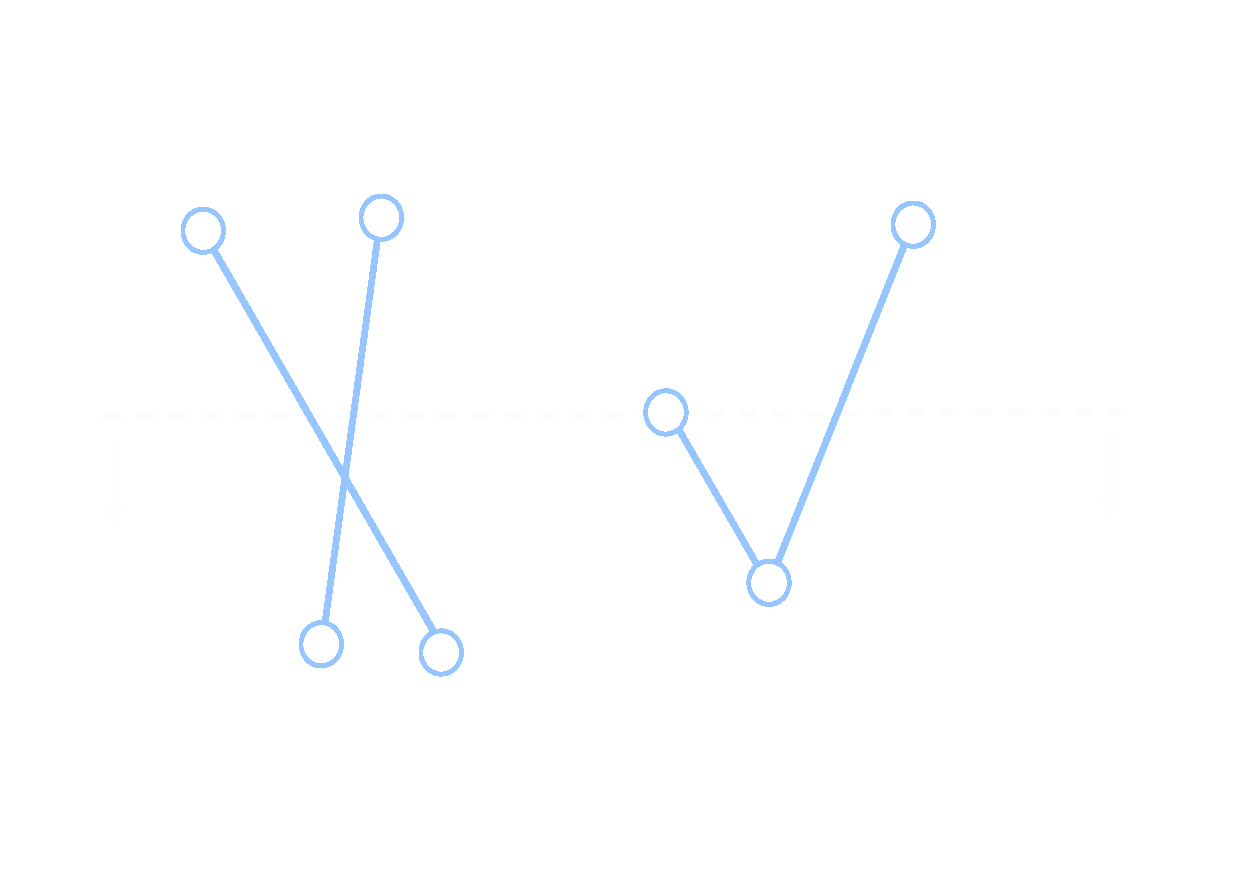
\includegraphics[width=0.6\textwidth]{картинки/нормкартинки/sweepline1.pdf}
	\end{center}
\end{frame}

\begin{frame}{Event points}
        Вершины, соответствующие концам отрезков,\\
        будем называть {\it крайними событиями,}\\
        а их пересечениям~— {\it внутренними событиями.}\\
        Упорядочим события следующим образом:
        \[ p \prec q\ \ \longleftrightarrow\ \ \left[ 
      \begin{gathered} 
        p_y > q_y \\ 
        p_y = q_y, \; p_x < q_x \\ 
      \end{gathered} 
       \right. \]
\end{frame}


\begin{frame}{Статус}
        \vphantom{x}{\it Статусом заметающей прямой} будем называть\\
        последовательность отрезков, пересекающих её\\
        в данный момент.

        \begin{center}
        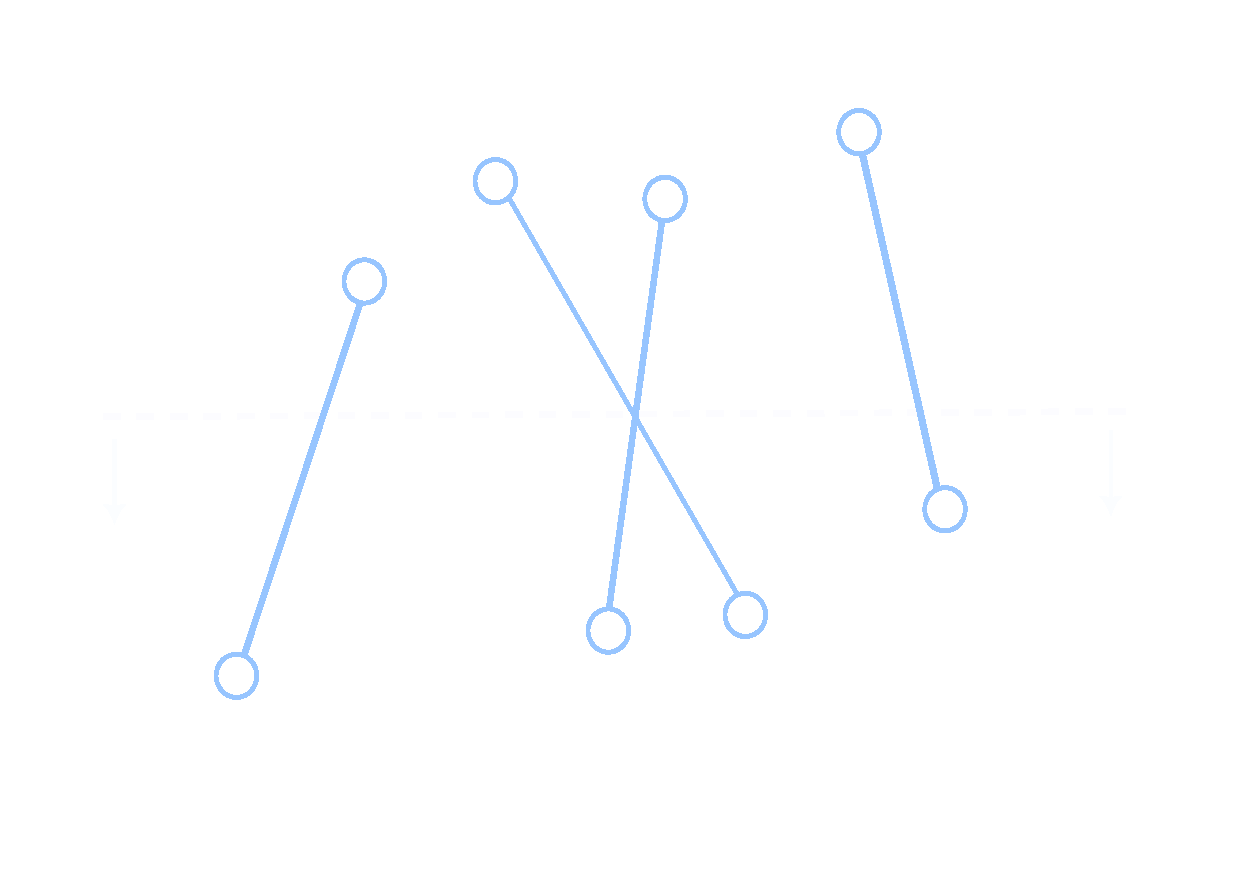
\includegraphics[width=0.5\textwidth]{картинки/нормкартинки/sweepline2.pdf}
	\end{center}
\end{frame}

\begin{frame}{Статус}
        \vphantom{x}{\it Статусом заметающей прямой} будем называть\\
        последовательность отрезков, пересекающих её\\
        в данный момент.

        \begin{center}
        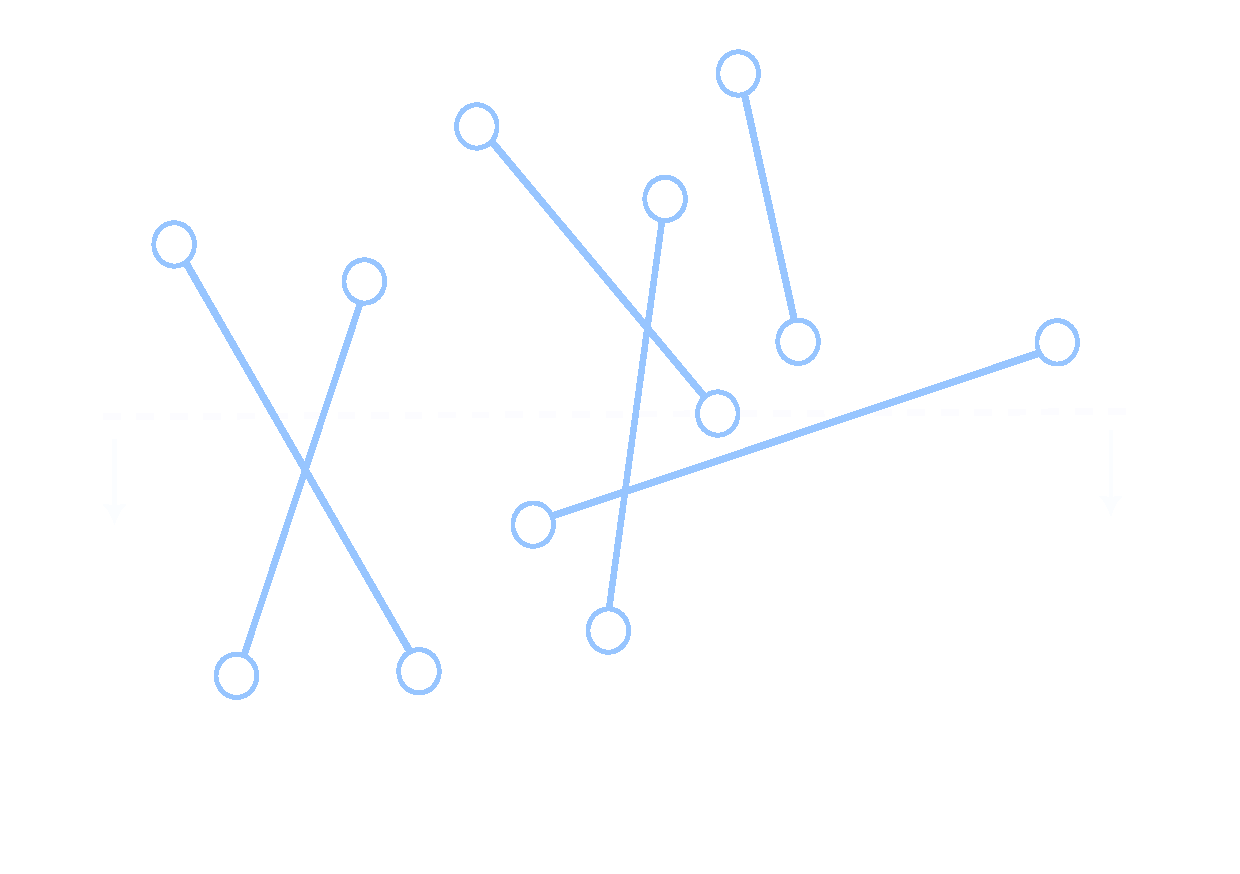
\includegraphics[width=0.5\textwidth]{картинки/нормкартинки/sweepline3.pdf}
	\end{center}
\end{frame}

\begin{frame}{Бинарное дерево статуса}
        Для хранения статуса используем бинарное дерево $T$. Оно\\ понадобится нам для нахождения ближайших к событию отрезков.

    \begin{center}
        \includegraphics[width=0.43\textwidth]%
          {картинки/нормкартинки/sweepline_for_tree.pdf}
        \ \ 
        \includegraphics[width=0.43\textwidth]%
          {картинки/нормкартинки/tree.pdf} 
    \end{center}
\end{frame}

\begin{frame}{Общий алгоритм}
        \begin{itemize}
            \item создаем пустую очередь $Q$ и заполняем ее\\
            крайними событиями (если событие --- верхняя вершина\\
            отрезка $s$, то кладем $s$ вместе с ней) 
            \item создаем пустое дерево статуса
            \item пока $Q \neq \varnothing$, определяем,
            какое событие будет следующим,\\
            удаляем текущее и обрабатываем следующее 
        \end{itemize}
\end{frame}

\begin{frame}{Обработка события}
    $U(p)$ --- отрезки, верхняя вершина которых $p$ \\ %см очередь, там они есть
    $L(p)$ --- отрезки, нижняя вершина которых $p$ \\
    $C(p)$ --- отрезки, содержащие $p$ внутри \medskip \\

 \begin{algorithmic}
    \If{$U(p) \cup L(p) \cup C(p) \neq \varnothing$}
        \State $p$ --- пересечение набора отрезков $U(p) \cup L(p) \cup C(p)$
    \EndIf
    \State удаляем отрезки из $L(p) \cup C(p)$
    \State добавляем отрезки из $U(p) \cup C(p)$
 \end{algorithmic}
\end{frame}

\begin{frame}{Обработка события}
 \begin{algorithmic}
    \If{$U(p) \cup C(p) = \varnothing$}
        \State находим соседей $p$ с помощью $T$ --- $s_l$, $s_r$
        \State $\text{FindNewEvent}\lr*{s_l,s_r,p}$
    \Else 
        \State $s' \coloneqq$ крайний левый в $U(p) \cup C(p)$
        \State $s_l \coloneqq$ слева от $s^{\prime}$
        \State $\text{FindNewEvent}\lr*{s_l,s^{\prime},p}$
        \State $s^{\prime\prime} \coloneqq$ крайний правый в $U(p) \cup C(p)$
        \State $s_r \coloneqq$ справа от $s^{\prime\prime}$
        \State $\text{FindNewEvent}\lr*{s^{\prime\prime},s_r,p}$
    \EndIf
\end{algorithmic} 
\end{frame}

\begin{frame}{Сложность}
    $O\lr*{n \cdot \log n}$ --- заполнение очереди

    Пока $Q \neq \varnothing$ ($\leq 2n+I$ раз) \\
    \qquad изменение очереди~— $O(\log n)$ \\
    \qquad изменение дерева статуса~—
        $O\lr*{\log n \cdot \left|U(p) \cup L(p) \cup C(p)\right|}$
        \vspace{-6mm}

   \[ \sum\limits_{p}|U(p) \cup L(p) \cup C(p)|\ \ =\ \ O(2n+I)\ \ =\ \ O(n+I) \]
   \vspace{-16mm}

  \begin{multline*}
     O\lr*{n \cdot \log n} + O\lr*{\lr*{2n+I} \cdot \log n} +
       O\lr*{\log n \cdot \sum\limits_{p}|U(p) \cup L(p) \cup C(p)|} = \\
       = O\lr*{\lr*{n+I}\cdot \log n}
  \end{multline*}
\end{frame}


\section{DCEL (de Berg et al., p. 29+10)}

\begin{frame}{Карта на плоскости}
Разбиение \(\br^2\) на маркированные области.
\begin{center}
\begin{tikzpicture}[scale=0.56,draw=dcelcolor]
	\placeDcel
	\bsobl{\placeDcelEdges}
\end{tikzpicture}
\end{center}
\end{frame}

\begin{frame}{Карта на плоскости}
В вершинах и в областях могут храниться разные данные.
\begin{center}
\begin{tikzpicture}[scale=0.56,draw=dcelcolor]
	\placeDcel
	\bsobl{
	  \fill[p9260u,opacity=0.42] (v5)--(v8)--(v12)--(v14)--(v15)--(v9)--cycle;
	  \fill[p9121u,opacity=0.42] (v10)--(v16)--(v15)--(v9)--cycle;
	  \fill[p9480u,opacity=0.42] (v10)--(v9)--(v6)--cycle;
	  \fill[p9584u,opacity=0.42] (v9)--(v6)--(v3)--(v5)--cycle;
	  \fill[p9480u,opacity=0.42] (v3)--(v5)--(v2)--(v1)--cycle;
	  \fill[p9121u,opacity=0.42] (v2)--(v4)--(v8)--(v5)--cycle;
	  \fill[p9480u,opacity=0.42] (v4)--(v8)--(v7)--cycle;
	  \fill[p9584u,opacity=0.42] (v7)--(v8)--(v12)--(v11)--cycle;
	  \fill[p9121u,opacity=0.42] (v12)--(v11)--(v13)--(v14)--cycle;
	  \placeDcelEdges
	}
\end{tikzpicture}
\end{center}
\end{frame}

\begin{frame}{Поддерживаемые операции}
\begin{itemize}
	\item Обход области против часовой стрелки: даны клетка и ребро,\\
	      перейти к следующему ребру. \medskip
	\item Обход вершины по часовой стрелке: даны вершина и ребро,\\
	      перейти к следующему ребру. \medskip
	\item Переход между клетками: даны клетка и ребро, указать\\
	      клетку «по ту сторону» ребра.
\end{itemize}
\end{frame}

\begin{frame}{Полурёбра}
Рассмотрим вместо каждого ребра его два направленных варианта.
\begin{center}
\begin{tikzpicture}[scale=0.56,draw=dcelcolor]
	\placeDcel
	\placeDcelArrows
\end{tikzpicture}
\end{center}
\end{frame}

\begin{frame}{Структура данных}
Запись для каждых вершины, ребра, области; и указатели: \begin{itemize}
	\item от каждого полуребра к предыдущему и следующему,
	\item между двумя полурёбрами одного ребра,
	\item между вершиной и смежными с ней рёбрами,
	\item между областью и её рёбрами.
\end{itemize} \begin{center} \begin{tikzpicture}[scale=0.56,draw=dcelcolor]
	\dnode{0,0}{1} \dnode{4,-0.5}{2} \dnode{6,3}{3} \dnode{0.5,4}{4}
   \bsobl{
	\draw[dgray] (v1)--(v2) \ninjanode{0.6}{s1} -- (v3) \ninjanode{0.4}{s2}
	             (v3)--(v4) \ninjanode{0.45}{m1} \ninjanode{0.625}{vn}
	             (v4)--(v1) \ninjanode{0.65}{m2};
   }
	\dconn12 \dconn23 \dconn34 \dconn41
	\draw[FireBrick,<->] (s1) to[out=90,in=150] (s2);
	\draw[FireBrick,<->] (m1) to[out=255,in=50] (2.5,1.5);
	\draw[FireBrick,<->] (vn) to[out=-150,in=-60] (vn4);
	\draw[rotate=-7.1,FireBrick,<->] (m2) .. controls ++(2,1.2) and ++(-2,1.2) .. (m2);
\end{tikzpicture} \end{center}
\end{frame}

\begin{frame}{Дополнительные операции}
Имея DCEL, легко построить DCEL для {\it двойственного графа.} \\
Скопируем записи вершин, это будут новые грани.
\begin{center} \begin{tikzpicture}[scale=0.56,draw=dcelcolor]
	\dnode{0,0}{1} \dnode{4,-0.5}{2} \dnode{6,3}{3} \dnode{0.5,4}{4}
	\dconn12 \dconn23 \dconn34 \dconn41
	\fnode{7,1}{1} \fnode{2.5,1.5}{2} \fnode{1.5,-1.5}{3}
	\draw[fill3,->] (fn1) to[bend right] node[pos=0.55,inner sep=0.2mm](ve1){ }
	   node[pos=0.78,inner sep=0.2mm](ns1){ } (fn2);
	\draw[fill3,->] (fn2) to[bend right] node[pos=0.27,inner sep=0.2mm](ns2){ }
	   node[pos=0.45,inner sep=0.2mm](ve2){ } (fn3);
	\draw[FireBrick,<->] (vn2) to[bend left] (ve1);
	\draw[FireBrick,<->] (vn2) to[bend right] (ve2);
	\draw[FireBrick,<->] (ns1) to[bend left] (ns2);
\end{tikzpicture} \end{center} \vspace{-3mm}
Чтобы соединять указателями полурёбра, будем хранить,\\
какие вершины мы уже обслужили.
\end{frame}

\begin{frame}{Разрезание и склеивание}
\begin{itemize}
	\item \(\dcsplit (f,v_1,v_2)\)~— разделить область \(f\) ребром \(v_1v_2\) на две новых.
	\item \(\dcmerge (f_1,f_2,e)\)~— стереть ребро \(e\), объединив между собой \\
	   области \(f_1\) и \(f_2\).
\end{itemize}
\begin{center} \begin{tikzpicture}[scale=0.56,draw=dcelcolor]
	\dnode{0,0}{1} \dnode{4,-0.5}{2} \dnode{6,3}{3} \dnode{0.5,4}{4}
	\dconn12 \dconn23 \dconn34 \dconn41
	\draw[fill3] (vn2)--(vn4);
\end{tikzpicture} \end{center} \vspace{-3mm}

	В худшем случае занимают время~\(O(n)\), потому что переделывать \\
	все указатели ребро~\(\leftrightarrow\) область.
\end{frame}

\begin{frame}{Ломти}
	Разделим области на \alert{маленькие} и \alert{большие}. Большие~— те,\\
	у которых больше \(\sqrt{n}\) вершин.

	Полурёбра маленьких областей будем хранить как есть, полурёбра\\
	больших областей объединим в \alert{ломти} по примерно \(\sqrt{n}\) подряд идущих. \bigskip

	{\footnotesize \textcolor{white!46!dgray}{Картинка на доске}}
\end{frame}

\begin{frame}{То же самое за polylog}
\begin{block}{Упражнение.}
	Убедитесь, что, если хранить полурёбра в структуре\\
	{\it link-cut tree,} можно делать операции split и merge\\
	в среднем за \(O\lr*{\text{polylog}\lr*{n}}\).
\end{block}
\end{frame}


\begin{frame}{Спасибо за внимание!}
	\tableofcontents
\end{frame}

\end{document}
